\documentclass[11pt, a4paper]{article}

\usepackage{style}

\author{Vladislav Mlejnecký}

\title{%
  Číslicové zpracování signálů\\
  \large Úloha číslo 2.\\
  Generování signálů v prostředí Matlab - 2}

\begin{document}

    \maketitle

    \section{Zadání}
    
    Podobně jako v prvním cvičení, kreslete do jednoho okna grafu (body 1 až 5) a jen „rozumný“ počet vzorků.
    \begin{enumerate}
        \item
        generujte a  nakreslete náhodný šumový signál s normálním rozdělením o délce 200 vzorků a vzorkovací frekvenci 8kHz, rozsah amplitudy od -1 do 1 (funkce randn)
        \item
        generujte a  nakreslete náhodný šumový signál s rovnoměrným rozdělením o délce 200 vzorků a vzorkovací frekvenci 8kHz, rozsah amplitudy od -1 do 1 (funkce rand)
        \item
        Vygenerujte  harmonický signál s amplitudou 1 o kmitočtu F1=400Hz a délce 200 vzorků a k signálu přičtěte signál o kmitočtu 2xF1, nakreslete harmonický signál a složený signál.
        \item
        K signálu podle bodu 3 přičtěte signál dle bodu 2, a nakreslete výsledek.
        \item
        Vytvořte a zobrazte signál obdélníkového průběhu o frekvenci F1 Hz, délce trvání 400 vzorků, vzorkovací frekvence 8kHz (funkce square), nakreslete a upravte osy tak, aby byl vidět obdélníkový průběh.
        \item
        Vytvořte při vzorkovacím kmitočtu fs=1000Hz a zobrazte dva kmitočtově blízké signály f1= 99 a f2=101Hz a komentuje nakreslený výsledek.
        \item
        Vytvořte při vzorkovacím kmitočtu fs=200Hz a zobrazte signál f1= 99  a opět komentuje nakreslený výsledek.
    \end{enumerate}
            
    \section{Výsledké grafy}
    
        \begin{figure}[H]
            \centering
            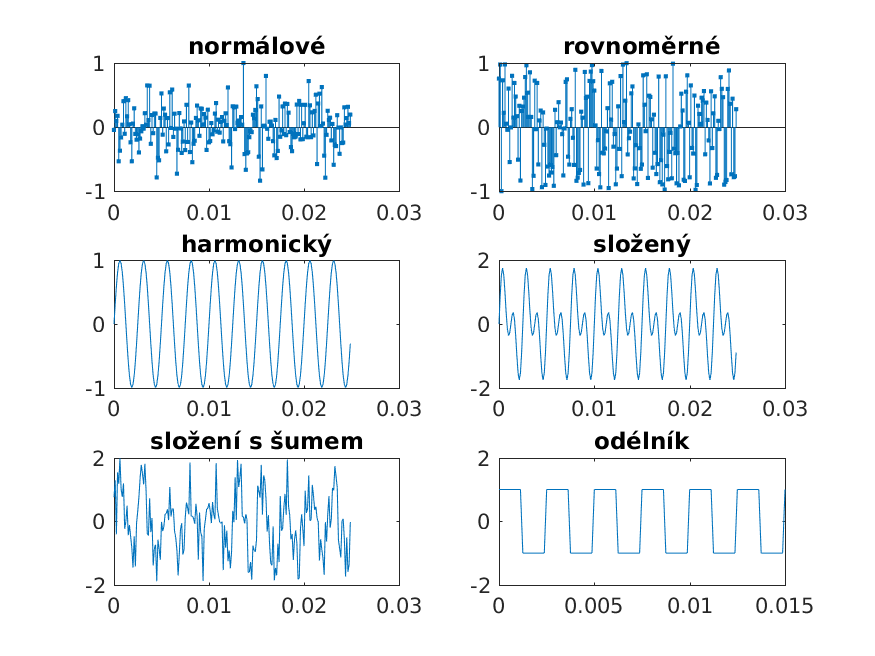
\includegraphics[width=.9\textwidth]{matlab/1.png}
            \caption{Různé druhy signálů}
            \label{fig:graf1}
        \end{figure}
        
        \begin{figure}[H]
            \centering
            \begin{minipage}{.5\textwidth}
                \centering
                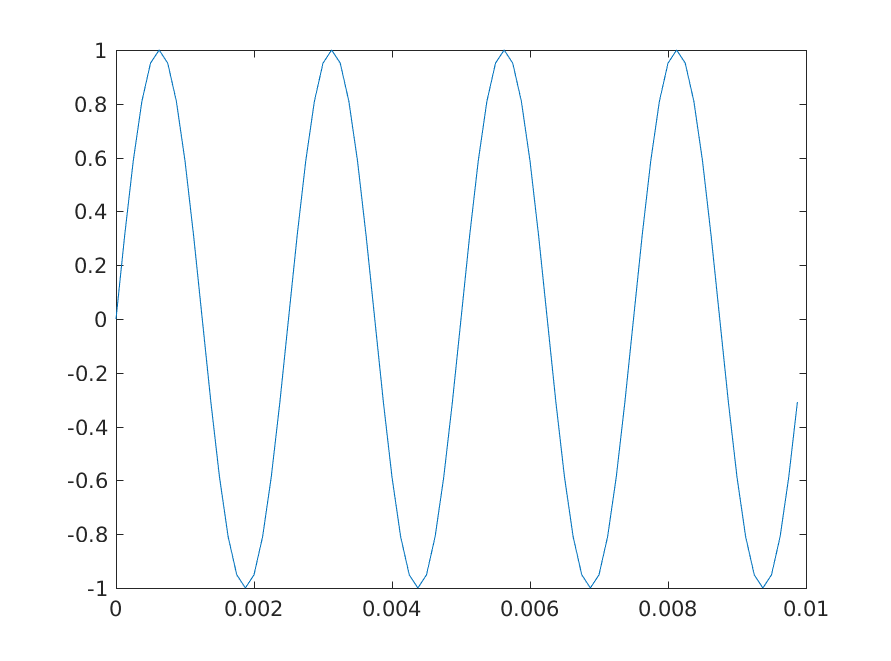
\includegraphics[width=.9\textwidth]{matlab/2.png}
                \caption{Dva blízké signály}
                \label{fig:graf2}
            \end{minipage}%
            \begin{minipage}{.5\textwidth}
                \centering
                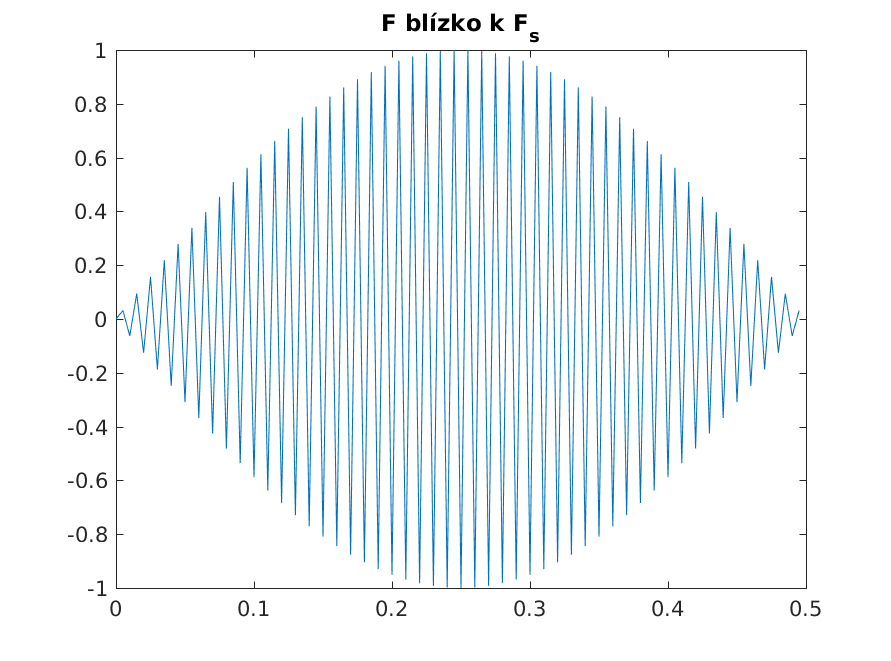
\includegraphics[width=.9\textwidth]{matlab/3.png}
                \caption{Signál frekvencí blízký vzorkovací}
                \label{fig:graf3}
            \end{minipage}
        \end{figure}
        
    \section{Komentář k výsledkům}
    
        Na obrázku \ref{fig:graf2} jsou dva signály, jeden o frekvenci 
        99Hz a druhý o frekvenci 101Hz. V dolní části obrázku je vidět 
        součet těchto signálů. Dochází zde k tzv. rázům, které jsou 
        způsobeny neceločíselným poměrem frekvencí obou signálů. 
        Frekvence rázů je dána vztahem \ref{eq:1}. V akustice se tyto 
        rázy někdy nazývají zázněje a jsou využívány k ladění hudebních 
        nástrojů.
        
        \begin{align}
            F_a &= \frac{F_1 - F_2}{2} \label{eq:1}
        \end{align}
        
        Na obrázku \ref{fig:graf2} je zachycena jiná situace, je zde 
        opět vzorkován signál o frekvenci 99Hz ale frekvence vzorkování 
        je snížena na 200Hz. Protože ale spektrum digitální signálu je 
        symetrické okolo celočíselných násobků vzorkovací frekvence 
        nastává stejný jev jako na obrázku \ref{fig:graf2}.
        
        \section{Výpis zdrojového kódu}
    
\begin{lstlisting}[language=matlab, frame=single]
h1 = figure();

Fs = 8000;

t = (0:199)*(1/Fs);
y1 = randn(1, 200);
y1 = y1./max(y1);
subplot(3, 2, 1);
stem(t, y1, '.');

y2 = rand(1, 200) * 2 -1 ;
subplot(3, 2, 2);
stem(t, y2, '.');

y3a = sin(2 * pi * 400 * t);
y3b = sin(2 * pi * 800 * t);
subplot(3,2,3);
plot(t, y3a);
subplot(3,2,4);
plot(t, y3a + y3b);

y4 = y3a + y2;
subplot(3,2,5);
plot(t, y4);


t = (0:399)*(1/Fs);
y5 = square(2 * pi * 400 * t);
subplot(3, 2, 6);
plot(t, y5);
a = axis;
a = [a(1) a(2)/4 2*a(3) 2*a(4)];
axis(a);

saveas(h1, '1.png');


h2 = figure();

Fs = 1000;
t = 0:1/Fs:0.5 - 1/Fs;

sine_a = sin(2 * pi * 99 * t); 
sine_b = sin(2 * pi * 101 * t); 
sine_c = sine_a + sine_b;

subplot(3, 1, 1);
plot(t, sine_a);
subplot(3, 1, 2);
plot(t, sine_b);
subplot(3, 1, 3);
plot(t, sine_c);

saveas(h2, '2.png');

h3 = figure();

Fs = 200;
t = 0:1/Fs:0.5 - 1/Fs;
y7 = sin(2 * pi * 99 * t); 

plot(t, y7);

saveas(h3, '3.png');
\end{lstlisting}
    
        
        
        

\end{document}
